%% S8: every infinite comb of closed S-terms has teeth of unbounded size.
%% DRAFT 2026-11-24 (skinock).  Neutral amsart shell, as S1--S7.
%% Sources: ~/Code/ski/notes/NCFP-proof.md (sections 0--3, 7.3 Prop. Rot, 8.1--8.3, 9.1) and the NCFP
%%          section of ~/Code/ski/notes/A1-lock1-S3.md (Lemma L, Theorem 2), with their Wizard reviews.
%% Paper-to-Lean map (lean-ski, branch ncfp, module Ski/Ncfp.lean, gate Ski/NcfpAudit.lean):
%%   lem:distinct ..... Ncfp.Desc.irrefl, Ncfp.desc_finite (from HeadRec.no_ground_loop)
%%   lem:frames (a) ... Ncfp.lemma_L, Ncfp.lemma_L', Ncfp.hnf1_literal
%%   lem:frames (b) ... Ncfp.last_item_step, Ncfp.link
%%   lem:frames (c) ... pending (Lemma P of the note)
%%   thm:comb, hnf combs ... pending in the mixed form (Theorem G of the note).  Special cases exist:
%%                      Ncfp.right_combs, right_combs_seq (teeth a_n only), Ncfp.first_combs,
%%                      first_combs_seq (teeth b_n only); SS-chains: Ncfp.ss_bound
%%   thm:comb, left combs .. Ncfp.teeth_unbounded, teeth_unbounded_seq; the moves: Ncfp.bmove, Ncfp.lemma_A
%%   lem:invariant .... S6's lemma (Conv); term level Ncfp.lemma_T, Ncfp.right_combs_conv, first_combs_conv
%%   cor:hnf .......... pending in the mixed form (Cor. G1 of the note).  Special cases exist:
%%                      Ncfp.ncfp_comb (S E, S n E), Ncfp.ncfp_fcomb (S E, S E n)
%%   cor:fpc .......... Ncfp.ncfp_S, Ncfp.no_fixed_point_combinator, Ncfp.no_fpc
%%   cor:left ......... the case without hnf: Ncfp.cor_B1, cor_B1'; normalizing case: Ncfp.prop0;
%%                      the cases S, S a (Prop. A of the note) and the rotation: pending
%% TODO before release (the Data availability section is written as if all of this were done):
%%   1. Ski/Ncfp.lean and Ski/NcfpAudit.lean are untracked files on branch ncfp: build them
%%      (lake build, read the log), commit, and merge after a Wizard pass.
%%   2. Mechanize the pending items above: lem:frames (c), the mixed hnf comb (thm:comb), cor:hnf in
%%      the mixed form, and the cases S, S a and the rotation of cor:left.  Put all in #audit_clean.
%%   3. If the Lean statement of thm:comb stays split (right_combs, first_combs, teeth_unbounded),
%%      either add the unified statement or reword Data availability.
%%   4. Release lean-ski with module Ncfp; update the version and URL in refs.bib (leanski), and
%%      the module name in Data availability if it changes.
%%   5. The note's section 9 (Lemma P, Theorem G, Cor. G1) has no dated Wizard line yet; record it.
%%   6. Grammarian on the prose; Wizard on this text (the unified proof of the hnf case merges
%%      Theorem 2 and Theorem G of the notes and is new as a text).
%%   7. polonsky: add the page range once checked on the LMCS page (volume, issue, paper number and DOI are checked).
%%   8. Figures: `make figs` regenerates fig/sasa.pdf and fig/zs.pdf (needs ~/Code/ski/notes/checks/s15/cert).
\documentclass[11pt]{amsart}
\usepackage[T1]{fontenc}
\usepackage{lmodern}
\usepackage{amsmath,amssymb,amsthm}
\usepackage{graphicx}
\usepackage[numbers,sort]{natbib}
\usepackage[hidelinks]{hyperref}
\usepackage{bm}

\newtheorem{theorem}{Theorem}
\newtheorem{lemma}[theorem]{Lemma}
\newtheorem{corollary}[theorem]{Corollary}
\newtheorem{conjecture}[theorem]{Conjecture}
\theoremstyle{definition}
\newtheorem{definition}[theorem]{Definition}

\newcommand{\Ter}{\mathcal S}
\newcommand{\red}{\twoheadrightarrow}
\newcommand{\hred}{\twoheadrightarrow_h}
\newcommand{\conv}{=_\beta}
\newcommand{\sz}[1]{\lvert#1\rvert}

\title{Infinite Combs of the Combinator $\bm{S}$ Have Unbounded Teeth}
\author{Claude Opus \& Fable with N.\ E.\ Davis}
\address{ZeroAttest, Champaign, Illinois, USA}
\email{NDavis@ZeroAttest.com}
\urladdr{https://orcid.org/0000-0002-1131-8319}
\date{\today}

\begin{document}
\begin{abstract}
A comb is a sequence of closed terms built from the combinator $S$ in which each term has the
next as an item of its head normal form, or as the function part of its first stable frame; the
items left behind are the teeth. We show that the teeth of an infinite comb are unbounded in size.
Hence no closed $S$-term $p$ is convertible with $E[p]$ for a context $E\ne[\,]$ built from the hole
by $E\mapsto S\,E$, $S\,n\,E$ and $S\,E\,n$ with $n$ normalizing, and no term without a head normal
form is convertible with itself applied to normalizing arguments. Statman's theorem that $S$
defines no fixed-point combinator is an instance. The proofs rest on the absence of ground loops.
\end{abstract}

\keywords{combinatory logic, combinator $S$, head reduction, fixed points, convertibility}
\maketitle

\section{Introduction}

$\Ter$ is the set of closed terms built from $S$ by application, with $S\,x\,y\,z\to x\,z\,(y\,z)$ at
any position; $\red$ is the reflexive--transitive closure of $\to$ and $\conv$ is convertibility. The
\emph{size} $\sz t$ is the number of occurrences of $S$ in $t$. A step never lowers the size, since
$z$ contains an $S$. A term is \emph{normalizing} if it reduces to a normal form $n$; every term convertible with it then reduces to $n$, by Church--Rosser, and has size at most $\sz n$.

Frames are those of~\citep{s6}. Every $t\in\Ter$ is $S\,u_1\cdots u_m$ for a unique $m\ge0$; this is
its \emph{frame}, the $u_i$ are its \emph{items}, and $t$ is a \emph{head normal form} (hnf) iff
$m\le2$. If $m\ge3$, the \emph{head step} is $t\to u_1\,u_3\,(u_2\,u_3)\,u_4\cdots u_m$. Head steps
define the \emph{head run} of $t$, and $\hred$ is its reflexive--transitive closure; $t$ \emph{has
an hnf} if its head run reaches one. A frame with $m\ge3$ is \emph{stable} if $S\,u_1\cdots u_{m-1}$
has no hnf; we write it $f\,w$ with $w=u_m$. The frames on the head run of a term $f$ without an hnf have at least three items, so the head
run of $f\,w$ is that of $f$ with $w$ appended: a stable frame has no hnf, and $g\,x$
is a stable frame whenever $g$ has no hnf. The head run of every term reaches an hnf or a stable
frame~\citep{s1,s3}.

No $t\in\Ter$ reduces in one or more steps to a term that contains
it~\citep{waldmann-ic,s7}: there are no \emph{ground loops}. From this we derive
Theorem~\ref{thm:comb}, and from it that certain equations $p\conv E[p]$ have no solution
(Section~\ref{sec:cor}).

\section{Combs}\label{sec:comb}

\begin{definition}\label{def:comb}
A \emph{comb} is a finite or infinite sequence $q_0,q_1,\dots$ in $\Ter$ with, for each $n$ that has a successor, one of the following.
\begin{itemize}
\item An \emph{hnf step}: $q_n$ has the hnf $S\,q_{n+1}$, $S\,a_n\,q_{n+1}$ or $S\,q_{n+1}\,b_n$.
\item A \emph{left step}: $q_n$ has no hnf, and the first stable frame on its head run is
  $q_{n+1}\,w_n$.
\end{itemize}
The terms $a_n$, $b_n$, $w_n$ are the \emph{teeth}. A comb of hnf steps is an \emph{hnf comb}, and a comb of left steps is a \emph{left comb}.
\end{definition}

A term without an hnf starts exactly one infinite comb, which is a left comb. After a left step, $q_{n+1}$ has no hnf, so every later step is a left step, and an infinite comb is an hnf comb or has a tail that is a left comb. We prove the following theorem for the two kinds in turn.

\begin{theorem}\label{thm:comb}
The teeth of an infinite comb are unbounded in size.
\end{theorem}

\begin{lemma}\label{lem:distinct}
The terms of a comb are pairwise distinct. Hence, for every $M$, only finitely many of them have
size at most $M$.
\end{lemma}

\begin{proof}
Each $q_n$ reduces to a term of which $q_{n+1}$ is a proper subterm, so for $i<j$ the term $q_i$
reduces to a term $u$ of which $q_j$ is a proper subterm. If $q_i=q_j$, then $u\ne q_i$, and
$q_i\to^+u$ is a ground loop, which does not exist~\citep{s7}.
\end{proof}

\begin{lemma}\label{lem:frames}
Let $F\to F'$ be a head step, where $F$ has $m\ge3$ items, the first being $u_1$.
\begin{itemize}
\item[(a)] $F'$ has $m-1$ items more than $u_1$, so at least two. Hence a head run that ends in $S$ or
  $S\,a$ has no step, and a head run of one or more steps to a two-item hnf ends with
  $S\,S\,y\,z\to S\,z\,(y\,z)$.
\item[(b)] $F$ and $F'$ have the same last item if $m\ge4$. If $m=3$, the last item of $F'$ is an
  application whose argument is the last item of $F$.
\item[(c)] If $F'=S\,S\,y\,a$, then $F=S\,S\,y'\,S\,a$ with $y=y'\,S$, or $F=S\,(S\,S)\,y'\,y$ with
  $a=y'\,y$.
\end{itemize}
\end{lemma}

\begin{proof}
The items of $F'=u_1\,u_3\,(u_2\,u_3)\,u_4\cdots u_m$ are those of $u_1$, then $u_3$, $u_2\,u_3$,
$u_4,\dots,u_m$. This gives (a), with $m=3$ and $u_1=S$ for two items, and (b). In (c), $F'$ has three
items, so $u_1=S$ and $m=4$, with $(u_3,u_2\,u_3,u_4)=(S,y,a)$, or $u_1=S\,S$ and $m=3$, with
$(u_3,u_2\,u_3)=(y,a)$.
\end{proof}

\begin{figure}[t]
\centering
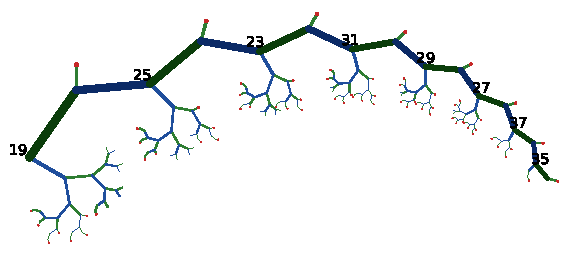
\includegraphics[width=0.72\textwidth]{fig/zs.pdf}
\caption{An hnf comb: the infinitary normal form~\citep{s3} of $Z\,S$, $Z=S\,T\,T\,(S\,T\,T)$,
$T=S\,S$, along its comb to depth 16, the teeth to depth 5. Function edges are green, argument
edges blue, leaves $S$ red. The comb is thick: $q_n$ has the hnf $S\,q_{n+1}\,b_n$, and the tooth
$b_n$ hangs on the thin blue edge, with its size $\sz{b_n}$ as a term. The comb
is infinite: the terms $r_n$ on the rightmost branch of $Z$ are $T^j(S\,T\,T)\,(T^k(S\,T\,T))$, and
$r_n\,S\hred S\,(r_{n+1}\,S)\,b_n$. By Theorem~\ref{thm:comb} the sizes are unbounded.}
\label{fig:zs}
\end{figure}

\begin{proof}[Proof of Theorem~\ref{thm:comb} for hnf combs]
Let $q_0,q_1,\dots$ be an infinite hnf comb with teeth of size at most $M$, where $M\ge1$. A tail
of a comb is a comb, so by Lemma~\ref{lem:distinct} we may assume $\sz{q_n}>M$ for all $n$. Call $n$
\emph{literal} if $q_n$ is an hnf; then $q_{n+1}$ is a proper subterm of $q_n$.

The \emph{last frame} of a term that has an hnf and is not one is the frame before the hnf on its head run.

(i) \emph{If $n$ is not literal, the last frame of $q_n$ is $S\,S\,y_n\,a_n$, and
$q_{n+1}=y_n\,a_n$.} By Lemma~\ref{lem:frames}(a) the last frame is $S\,S\,y\,z$ and the hnf is
$S\,z\,(y\,z)$. If $q_{n+1}$ were $z$, the tooth would be $y\,z$, which is larger than $q_{n+1}$; but $\sz{q_{n+1}}>M$.

(ii) \emph{If $n$ is not literal and $n+1$ is, then $y_n=S\,q_{n+2}$.} The hnf $q_{n+1}=y_n\,a_n$ is
$S\,q_{n+2}$, $S\,a_{n+1}\,q_{n+2}$ or $S\,q_{n+2}\,b_{n+1}$. The first two give $q_{n+2}=a_n$, which is excluded by size.

(iii) \emph{If $n,\dots,n+r$ are not literal and $n+r+1$ is, then $q_{n+r+2}$ is a proper subterm of
$q_n$.} Let $u=q_{n+r+2}$, $g_0=S\,u$, $g_{i+1}=S\,S\,g_i$ and $a=a_{n+r}$. No $g_i$ is of the form
$y'\,S$, since $u\ne S$ and $g_i\ne S$, and $\sz{g_i}>\sz u>M\ge\sz a$. By Lemma~\ref{lem:frames}(c), no head step leads to
$S\,S\,g_i\,a$, so a term with this last frame is this frame. By (i) and (ii) the last
frame of $q_{n+r}$ is $S\,S\,g_0\,a$, so $q_{n+r}=S\,S\,g_0\,a$. If $q_{n+r-i}=S\,S\,g_i\,a$ and
$i<r$, then by (i) it is $y_{n+r-i-1}\,a_{n+r-i-1}$, so the last frame of $q_{n+r-i-1}$ is
$S\,S\,g_{i+1}\,a$, and $q_{n+r-i-1}=S\,S\,g_{i+1}\,a$. Hence $q_n=S\,S\,g_r\,a$, which contains $u$.

(iv) \emph{From some $n$ on, no index is literal.} Otherwise every maximal run of non-literal indices is finite. Let $n_0=0$, and let
$n_{k+1}=n_k+1$ if $n_k$ is literal, and $n_{k+1}=n_k+r+2$ if $n_k,\dots,n_k+r$ is a maximal run of
non-literal indices. Then $q_{n_{k+1}}$ is a proper subterm of $q_{n_k}$ for all $k$, by (iii) and the remark on literal indices, which is impossible.

(v) \emph{There is a sequence $g_0,g_1,\dots$ with $g_n\hred S\,S\,g_{n+1}$ for all $n$.} Drop the
terms before the $n$ of (iv). By (i), the head run of $q_{n+1}=y_n\,a_n$ leads to the frame
$S\,S\,y_{n+1}\,a_{n+1}$. By Lemma~\ref{lem:frames}(b), $a_{n+1}$ is $a_n$ or properly contains it. The sizes are bounded, so $a_n$ is
a fixed term $a$ from some $n$ on, and then the frames from $y_n\,a$ to $S\,S\,y_{n+1}\,a$, except the last,
have at least four items. Their head steps are head steps of the frame without its last item $a$,
so $y_n\hred S\,S\,y_{n+1}$.

(vi) \emph{There is no such sequence.} We use strong induction on $\sz{g_0}$. If $g_0=S\,S\,g_1$,
then $g_1$ starts a sequence and is smaller. Otherwise the last frame of $g_0$ is $S\,S\,y_0\,S$ and
$g_1=y_0\,S$, by Lemma~\ref{lem:frames}(a). If $g_n=y_{n-1}\,S$ with $n\ge1$, then
$g_n\ne S\,S\,g_{n+1}$, since $S$ has no hnf $S\,S\,g_{n+2}$; so the last frame of $g_n$ is $S\,S\,y_n\,S$ and
$g_{n+1}=y_n\,S$. By Lemma~\ref{lem:frames}(b), the last item of these last frames, which is not an application, is the last item throughout
the head run. So $g_0=G\,S$, and, as in (v), $G\hred S\,S\,y_0$ and $y_{n-1}\hred S\,S\,y_n$ for $n\ge1$. The sequence $G,y_0,y_1,\dots$ starts with a
smaller term than $g_0$.
\end{proof}

\begin{lemma}[moves]\label{lem:moves}
Let $f=g\,u$ have no hnf, and let $f'\,w$ be the first stable frame on its head run. If $g$ has
no hnf, then $f'=g$ and $w=u$. Otherwise there are $k\ge0$ and terms $a_i$, $b_i$, $w_i$ with
$w_0=u$, $w_{i+1}=b_i\,w_i$, $f'=a_k\,w_k$, $w=w_{k+1}$ and
\[
  g\hred S\,a_0\,b_0,\qquad a_i\,w_i\hred S\,a_{i+1}\,b_{i+1}\quad(i<k).
\]
\end{lemma}

\begin{proof}
If $g$ has no hnf, $f$ is a stable frame. Otherwise the head run of $f$ follows that of $g$, with
$u$ appended, to the hnf of $g$. This hnf has two items, as $f$ has no hnf: $f\hred S\,a_0\,b_0\,w_0$. In general, from
$S\,a_i\,b_i\,w_i$ a head step gives $a_i\,w_i\,w_{i+1}$. If $a_i\,w_i$ has no hnf, this is a stable frame; put $k=i$.
Otherwise the run follows that of $a_i\,w_i$ to its hnf, which again has two items, and reaches
$S\,a_{i+1}\,b_{i+1}\,w_{i+1}$. No frame passed before is stable: in each, the frame without the last item has an hnf. Since the run reaches a stable frame, some $k$ occurs.
\end{proof}

\begin{figure}[t]
\centering
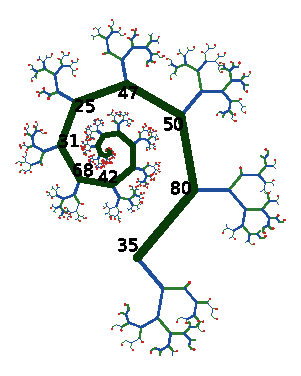
\includegraphics[width=0.42\textwidth]{fig/sasa.pdf}
\caption{A left comb: the infinitary normal form of $S\,A\,S\,A$, $A=S\,S\,S$, which has no hnf, to
depth 20, the teeth to depth 6; colours as in Figure~\ref{fig:zs}. The thick spiral is the infinite
left spine of the root. Its arguments are the infinitary normal forms of the teeth
$w_0,w_1,\dots$~\citep{s3}; the numbers are the sizes $\sz{w_n}$ of the teeth as terms, $n<8$. By
Theorem~\ref{thm:comb} they are unbounded.}
\label{fig:sasa}
\end{figure}

\begin{proof}[Proof of Theorem~\ref{thm:comb} for left combs]
Let $q_0,q_1,\dots$ be a left comb with teeth of size at most $M$. For $f=g\,u$ put $\|f\|=\sz g$. Consider the
step from $f=q_n$ to $f'=q_{n+1}$ in the notation of Lemma~\ref{lem:moves}.

If $g$ has no hnf, then $f'=g$ and $\|f'\|<\sz g=\|f\|$.

Otherwise call $i\le k$ \emph{literal} if no head step is taken to $S\,a_i\,b_i$: then
$g=S\,a_0\,b_0$ if $i=0$, and $a_{i-1}=S\,a_i$ if $i\ge1$. If $i$ is not literal, then $\sz{a_i}<\sz{b_i}$, by
Lemma~\ref{lem:frames}(a). If every $i\le k$ is literal, $a_k$ is a proper subterm of $g$, and
$\|f'\|=\sz{a_k}<\|f\|$. If not, let $i$ be the last index that is not literal. The tooth $w_{k+1}$
contains $b_i\,w_i$, so $\sz{a_k}\le\sz{a_i}<\sz{b_i}<M$. Also $\sz{w_k}<\sz{w_{k+1}}\le M$. So
$\sz{f'}=\sz{a_k}+\sz{w_k}<2M$.

Since $\|q_n\|$ cannot fall forever, infinitely many $q_n$ have size less than $2M$, against
Lemma~\ref{lem:distinct}.
\end{proof}

\section{Equations without solutions}\label{sec:cor}

A \emph{context} $E$ is a term with holes $[\,]$, and $E[p]$ is $E$ with $p$ in every hole. The next lemma is the conversion invariance
of the observable of~\citep{s6}, taken over the model of terms modulo $\conv$, which maps to the 38-element model of~\citep{s1} by the block of a term.

\begin{lemma}[\citep{s6}]\label{lem:invariant}
Let $t\conv t'$. If the head run of $t$ reaches the hnf $S\,u_1\cdots u_m$, then that of $t'$ reaches an hnf $S\,u'_1\cdots u'_m$
with $u_i\conv u'_i$ for all $i$. If $t$ has no hnf, then $t'$ has none, and the first stable
frames $f\,w$ and $f'\,w'$ on their head runs satisfy $f\conv f'$ and $w\conv w'$.
\end{lemma}

\begin{corollary}\label{cor:hnf}
Let $E\ne[\,]$ be a context with one hole, built from the hole by $E\mapsto S\,E$,
$E\mapsto S\,n\,E$ and $E\mapsto S\,E\,n$ with $n\in\Ter$ normalizing. Then no $p\in\Ter$ satisfies
$p\conv E[p]$.
\end{corollary}

\begin{proof}
Let $E=K_1[\cdots K_m[\,]\cdots]$ with each $K_i$ of the form $S\,[\,]$, $S\,n\,[\,]$ or
$S\,[\,]\,n$, and let $E_i=K_{i+1}[\cdots K_m[\,]\cdots]$, so that $E_0=E$ and $E_m=[\,]$. Suppose
$p\conv E[p]$. We build an hnf comb with $q_0=p$ and $q_j\conv E_i[p]$ for $i<m$, $i\equiv j\pmod m$.
The term $E_i[p]$ is an hnf with the item $E_{i+1}[p]$ and at most one other item $n$. By
Lemma~\ref{lem:invariant}, $q_j$ has an hnf of the same form; let $q_{j+1}$ be its item
convertible with $E_{i+1}[p]$, where $E_m[p]=p\conv E_0[p]$. The tooth, if any, is convertible with
$n$, so its size is at most that of the normal form of $n$. This contradicts
Theorem~\ref{thm:comb}.
\end{proof}

\begin{corollary}[{Statman~\citep[Rem.~15]{dots}}]\label{cor:fpc}
No $Y\in\Ter$ satisfies $Y\,x\conv x\,(Y\,x)$ for all $x\in\Ter$.
\end{corollary}

\begin{proof}
For $x=S$ this is $p\conv S\,p$ with $p=Y\,S$, the case $E=S\,[\,]$ of Corollary~\ref{cor:hnf}.
\end{proof}

\begin{corollary}\label{cor:left}
Let $p\conv p\,x_1\cdots x_k$ with $k\ge1$ and $x_1,\dots,x_k\in\Ter$ normalizing. Then each of the
terms $p\,x_1\cdots x_i$, $0\le i\le k$, has an hnf with two items and no normal form. In particular,
$p\not\conv p\,x_1\cdots x_k$ if $p$ has no hnf.
\end{corollary}

\begin{proof}
Let $q=p\,x_1\cdots x_i$. Applying both sides to $x_1,\dots,x_i$ gives
$q\conv q\,x_{i+1}\cdots x_k\,x_1\cdots x_i$. So it suffices to consider $q\conv q\,y_1\cdots y_k$
with the $y_j$ normalizing.

If $q$ has a normal form $n$, then $n\,y_1\cdots y_k\conv n$ reduces to $n$, but it is larger.

If $q$ is $S$ or $S\,a$, then $q\,y_1\cdots y_k$ has more items than $q$. It is an hnf, or its head run takes a step and
its hnf, if any, has two items, by Lemma~\ref{lem:frames}(a). Each case contradicts Lemma~\ref{lem:invariant}. By
Lemma~\ref{lem:frames}(a), no other term has an hnf with fewer than two items.

If $q$ has no hnf, let $w_0,w_1,\dots$ be the teeth of its comb. The comb of $q\,y_1\cdots y_k$ passes
through $q\,y_1\cdots y_i$, $i=k,\dots,0$, and continues with the comb of $q$; its teeth are
$y_k,\dots,y_1,w_0,w_1,\dots$. By Lemma~\ref{lem:invariant} and induction, corresponding teeth of the
two combs are convertible: $w_n\conv y_{k-n}$ for $n<k$, and $w_{n+k}\conv w_n$. So every $w_n$ is
convertible with some $y_j$, and the teeth are bounded in size, against Theorem~\ref{thm:comb}.
\end{proof}

\section{Closing}\label{sec:close}

The combinators $X$ and $W$ with $X\,x\,y\,z\to x\,z\,(y\,z)\,z$ and $W\,x\,y\to x\,y\,y$ have
ground loops, and these give solutions of equations $p\conv E[p]$:
\begin{gather*}
X\,X\,X\,X\to X\,X\,(X\,X)\,X\to X\,X\,(X\,X\,X)\,X\to X\,X\,(X\,X\,X\,X)\,X,\\
W\,W\,(W\,W)\to W\,(W\,W)\,(W\,W)\to W\,W\,(W\,W)\,(W\,W).
\end{gather*}
So $p\conv X\,X\,p\,X$ for $p=X\,X\,X\,X$, and $p\conv p\,(W\,W)$ for $p=W\,W\,(W\,W)$, an equation of the kind of Corollary~\ref{cor:left}.

Corollary~\ref{cor:hnf} does not cover contexts with two holes, such as $S\,[\,]\,[\,]$, or teeth
without a normal form, and Corollary~\ref{cor:left} leaves open the terms with a two-item hnf.
Terms with a normal form satisfy the following~\citep{s7}.

\begin{conjecture}\label{conj:ncfp}
No $p\in\Ter$ and context $E\ne[\,]$ with at least one hole satisfy $p\conv E[p]$.
\end{conjecture}

\noindent A relative in the $\lambda$-calculus is Statman's conjecture that no fixed-point
combinator $Y$ satisfies $Y\conv Y\,\delta$, where $\delta=\lambda yx.\,x\,(y\,x)$.
Intrigila~\citep{intrigila} published a proof; a gap in it was reported later~\citep{polonsky}, and
we treat the conjecture as open.

\section*{Data availability}
\sloppy
Every result of this paper is proved in the Lean~4~\citep{lean4} development
\texttt{lean-ski}~\citep{leanski}, module \texttt{Ncfp}, using only the axioms \texttt{propext} and
\texttt{Quot.sound}; Lemma~\ref{lem:invariant} and the absence of ground loops are those
of~\citep{s6,s7}. Theorem~\ref{thm:comb} is stated there for a set of terms closed under the steps of
Definition~\ref{def:comb} rather than for a sequence, so that no choice is needed. The figures are
drawn by \texttt{fig/spiral.py}, which computes prefixes of infinitary normal forms as
in~\citep{s3} and the teeth from the head runs.

\bibliographystyle{plainnat}
\bibliography{refs}
\end{document}
